\documentclass[a4,10pt]{article}
\usepackage{pgfplotstable}
\usepackage{booktabs}
\usepackage{setspace}
\usepackage{xeCJK}
\usepackage{mathptmx}
\usepackage{anyfontsize}
\usepackage{t1enc}
\usepackage{graphicx}
\usepackage[top=20mm,bottom=20mm,left=20mm,right=20mm]{geometry}
\usepackage{wrapfig}
\usepackage{float} %设置图片浮动位置的宏包
\usepackage{subfigure} %插入多图时用子图显示的宏包
\usepackage[justification=centering]{caption}
\usepackage{ctex}
\usepackage{minted}
\usemintedstyle{borland}
\usepackage{xcolor}
\usepackage[
backend=biber,
style=nature,
]{biblatex}


\addbibresource{citation.bib}

\makeatletter
  \def\vhrulefill#1{\leavevmode\leaders\hrule\@height#1\hfill \kern\z@}
\makeatother

\pagestyle{plain}

\begin{document}
\begin{titlepage}
    \begin{center}
 %       \includegraphics[scale=0.5]{Figure/SCU.png}\\
        

        \vspace{1.5cm}

        \textbf{\zihao{1}\songti{西\hspace{1cm}安\hspace{1cm}交\hspace{1cm}通\hspace{1cm}大\hspace{1cm}学\hspace{1cm}验\hspace{1cm}报\hspace{1cm}告}}\\

        \vspace{1cm}

   %     \includegraphics[scale=0.5]{Figure/SCU_logo.png}\\

        \vspace{2cm}

        \begin{tabular}{ll}
            \zihao{4}\songti{实\hspace{0.5em}验\hspace{0.5em}名\hspace{0.5em}称:\hspace{0.5em}\underline{教学计划编制程序\hspace{1em}}} & \zihao{4}\songti{课\hspace{0.5em}程\hspace{0.5em}名\hspace{0.5em}称:\underline{数据结构与算法\hspace{3em}}} \\
            \\
            \zihao{4}\songti{所\hspace{0.5em}在\hspace{0.5em}学\hspace{0.5em}院:\hspace{0.5em}\underline{抄作业学院\hspace{4em}}} & \zihao{4}\songti{专\hspace{3.5em}业:\underline{不知道\hspace{3em}}}\\
            \\
            \zihao{4}\songti{学\hspace{0.5em}生\hspace{0.5em}姓\hspace{0.5em}名:\underline{哈哈哈\hspace{5em}}} & \zihao{4}\songti{学\hspace{3.5em}号:\underline{111111111\hspace{1.5em}}}\\
            \\
             \zihao{4}\songti{班\hspace{3.5em}级:\underline{不愿意001\hspace{5em}}} & \zihao{4}\songti{实\hspace{0.5em}验\hspace{0.5em}日\hspace{0.5em}期:\underline{2024年6月1日\hspace{4em}}}\\
            \\

        \end{tabular}

        \vspace{3.2cm}
\begin{center}   
    \textbf{\zihao{4}{诚信承诺:我保证本实验报告中的程序和本实验报告是我自己编写,绝无抄袭。}}
\end{center}
        \vspace{2.4cm}
        \zihao{4}\songti{二〇二四年六月}

    \end{center}
\end{titlepage}


\renewcommand{\contentsname}{\centering 目录}  
\begin{spacing}{2}
\tableofcontents
\end{spacing}

\newpage
\section{实验目的}
\begin{enumerate}
\item{掌握拓扑排序,熟悉图的存储结构}
\item{掌握debug的逐过程和单步调试}
\item{初步掌握\LaTeX{}的写作方法}
\end{enumerate}
\subsection{问题图示}
\begin{figure}[h]
    \centering
    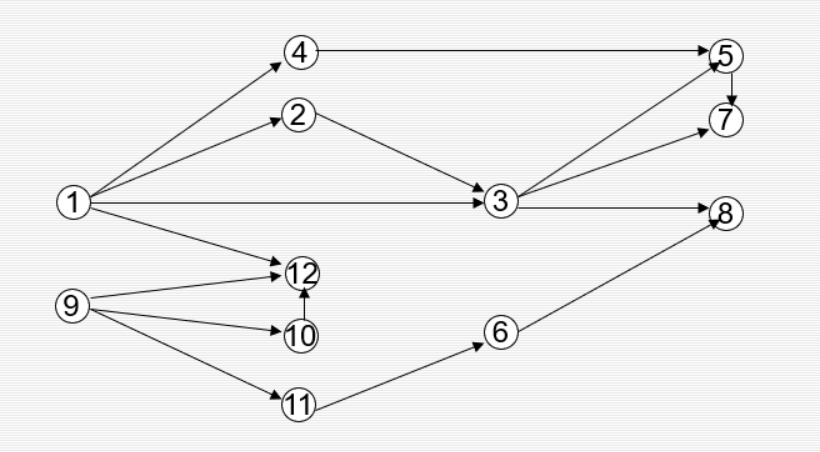
\includegraphics[width=0.8\textwidth]{quest.png}
    \caption{问题图示}
    \label{fig:question}
\end{figure}

\section{实验环境}
\textbf{硬件配置:}
\begin{enumerate}
    \item 处理器	AMD Ryzen 9 7940H w/ Radeon 780M Graphics,4001 Mhz,8 个内核,16 个逻辑处理器
    \item  已安装的物理内存(RAM)	16.0 GB
    \item 系统型号 $ASUS TUF Gaming A15FA507XV_FA507XV$
    
  
\end{enumerate}

\hspace{0.1em}\textbf{软件配置:} Visual Studio Code 

\section{项目设计和实现}
  \subsection{项目框架}
\begin{figure}[h]
    \centering
    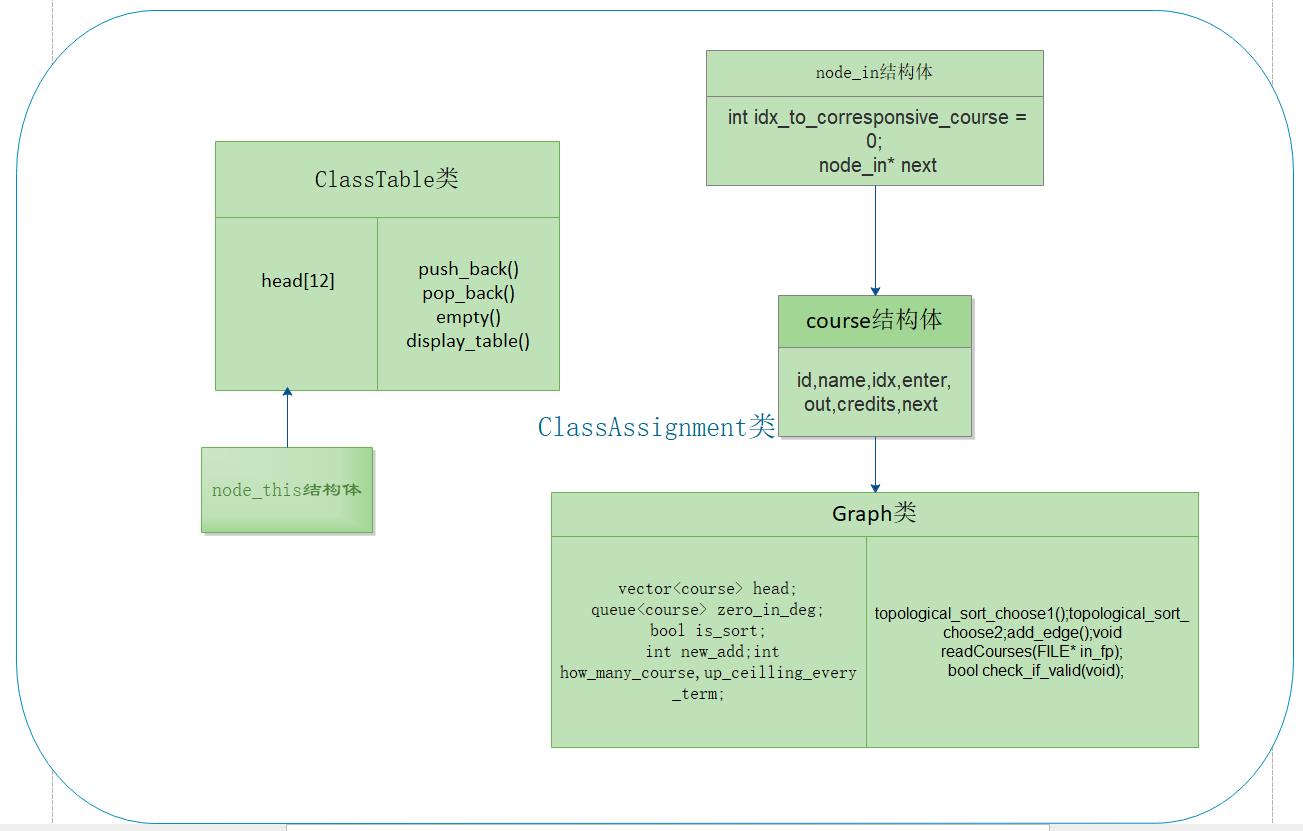
\includegraphics[width=0.9\textwidth]{6021.png}
    \caption{项目框架}
    \label{fig:enter-label}
\end{figure}
    
    \subsection{核心代码阐释}
    巧妙的是,本次主函数非常的简洁,除此之外ClassAssignment类也只有一个run()函数。
        \subsubsection{主函数}
        \begin{minted}
        [
        frame=lines,
        framesep=2mm,
        linenos,
        fontsize=\footnotesize,
        ]{C++}
     #include <iostream>
     #include "ClassAssignment.h"
using namespace std;
int main()
{
        ClassAssignment program;
        program.run();
        return 0;
}
        \end{minted}
        \subsubsection{Graph类的参数和一般方法}
\begin{enumerate}
\item{参数:vector<course> head为邻接表头节点,head[i] 是第 i 节课;queue<course> zero\_in\_deg来存储入度为0的结点;is\_sort 代表是否执行过拓扑排序;int new\_add代表每次拓扑排序后,zero\_in\_deg中新增的入度为零的节点,可以用于下次排序。}

\item{方法:topological\_sort\_choose1和topological\_sort\_choose2分别代表对应题目要求的两种不同策略的拓扑排序,readCourses(FILE* in\_fp)用于从记事本中读取信息存入head中,add\_edge()函数则构建起边的连接,采用的是邻接表的存储方式。对于该邻接表中的某个节点A,其node\_in* next的next相互连接,共同构成以A为先修条件的下一组课程(可能先修条件不仅仅只有A)。因为在拓扑排序的过程中,原有图的结构会产生破坏,因而check\_if\_valid(void)用于遍历所有course节点的入度,判断入度是否都为零,即可以认为检查拓扑排序的图是否存在环。}
\begin{figure}[h]
    \centering
    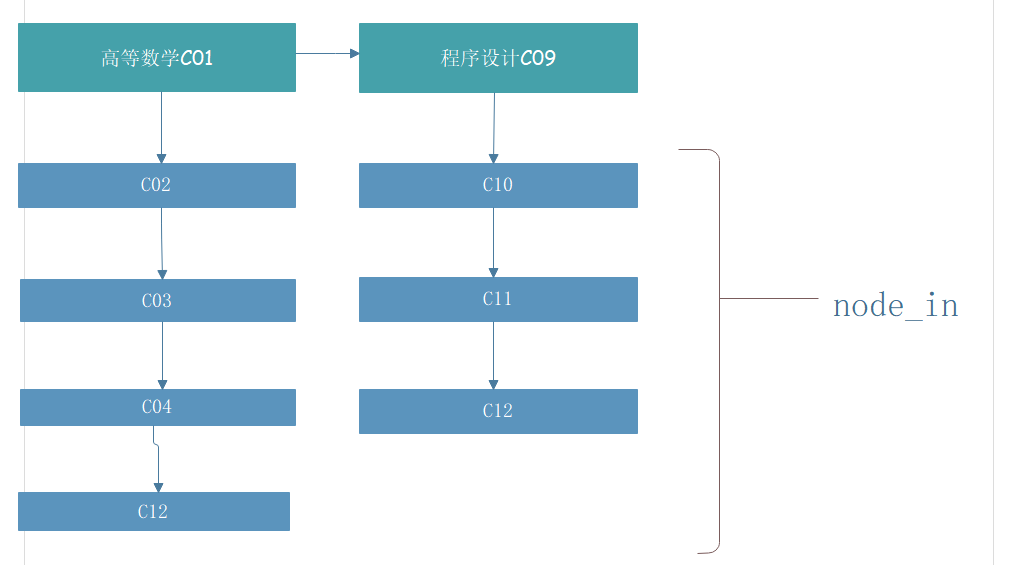
\includegraphics[width=0.8\textwidth]{6022.png}
    \caption{邻接表图示}
    \label{fig:show}
\end{figure}

\end{enumerate}
        \begin{minted}
        [
        frame=lines,
        framesep=2mm,
        linenos,
        fontsize=\footnotesize,
        ]{C++}
class Graph{
public:
       int how_many_course,up_ceilling_every_term;
       vector<course> head; //邻接表头节点,head[i] 是第 i 节课
       queue<course> zero_in_deg; //存储入度为0的结点
        bool is_sort = false; //是否执行过拓扑排序
  int new_add = -1;
  Graph()
       {
        cout<<"请输入一共要学多少门课程 , 以及每学期的学分上限:"<<endl;
        cin>>how_many_course>>up_ceilling_every_term;
        cout<<"---------------------------------成功-------------------------------------"<<endl;
        cout<<"---------------------------C:\\Users\\xixiboliya\\Desktop\\course.txt----------------------"<<endl;
        };
        void topological_sort_choose1(int xuefen,int term,ClassTable& class_table); //拓扑排序,均匀
        void topological_sort_choose2(int xuefen,int term,ClassTable& class_table); //拓扑排序,集中
       void add_edge(string num, vector<string> prerequisite); //添加一条有向边到图中,num 是该节点的课序号,prerequsite 是先置课程的序号
       void readCourses(FILE* in_fp);
  bool check_if_valid(void);
};

        \end{minted}
 
        \subsubsection{ClassTable类的参数和一般方法}
        ClassTable用于存放最终每学期所排的课程,node\_this head[12]中,head[i] 上挂的是第 i+1 学期的课程,采用邻接表存储方式,每一个head[i]中每一个是一个虚拟节点,data为空,其每一个虚拟节点的next接出该学期应该的所修课程。
        \begin{minted}
        [
        frame=lines,
        framesep=2mm,
        linenos,
        fontsize=\footnotesize,
        ]{C++}
   class ClassTable
{
public:
	node_this head[12]; //表头,head[i] 上挂的是第 i+1 学期的课
  ClassTable() {
    for (auto &i : head) {
        i = node_this();   //进行初始化,并使用了虚拟头节点。
    }
  }
  void push_back(int term, string name) //尾插法
  {
    node_this* tmp_ptr = &head[term];
    while (tmp_ptr->next)
    tmp_ptr = tmp_ptr->next; //寻找尾节点
    tmp_ptr->next = new node_this; //开辟新空间
    tmp_ptr->next->data=name;
  }
void pop_back(int term, string name) //尾部弹出一个结点
  {
    node_this* tmp_ptr = &head[term];
    node_this* tmp_ptr_previous = tmp_ptr;
    while (tmp_ptr->next)
    {
      tmp_ptr_previous = tmp_ptr;
      tmp_ptr = tmp_ptr->next; //找尾节点
    }
    if (tmp_ptr != &head[term])
    {
    name=tmp_ptr->data; //取出课程名
    if (tmp_ptr != &head[term])
     {
        delete tmp_ptr; //释放空间
        tmp_ptr_previous->next = nullptr; //防止野指针
    }
    }
   }
   bool empty(int term)
  {
    return (bool)(!(head[term].next));
    }
	void display_table(int terms)
  {
	  for(int i = 0;i <= terms ; i++)
    {
     cout<<"第"<<i+1<<"学期课程如下: "<<endl;
     node_this* ptr= head[i].next;
     while(ptr!=nullptr)
     {
        cout<<ptr->data<<endl;
        ptr=ptr->next;
      } 
    }
   }
};
        \end{minted}
          \subsubsection{Graph类add\_edge()函数的使用}
    这个函数是readCourses(FILE *in\_fp)之后调用的,作用在于建立一个以<course>为主主体的vector数组,并采用邻接表的形式存储,笔者精力憔悴,不想
        \begin{minted}
        [
        frame=lines,
        framesep=2mm,
        linenos,
        fontsize=\footnotesize,
        ]{C++}
void Graph::add_edge(string num, vector<string> prerequisite)
{
  int class_idx = (num[1] - '0') * 10 + num[2] - '0' - 1; // 获得欲添加的课程在 head 数组中的位置
  head[class_idx].idx = class_idx;      // 把课程号作为下标写入
  for (auto &pre : prerequisite)
  {
    head[class_idx].enter++; // 节点入度++
    int pre_idx = (pre[1] - '0') * 10 + pre[2] - '0' - 1;
    head[pre_idx].out++;       // 结点出度++
    node_in *cur_ptr = head[pre_idx].next; // 在前置课程的邻接表尾部插入当前课程
    if (!cur_ptr)
    {
      // 邻接表当前行只有头节点
      head[pre_idx].next = new node_in; // 添加新节点
      head[pre_idx].next->idx_to_corresponsive_course = class_idx;
    }
    else
    {
      while (cur_ptr->next)
      	cur_ptr = cur_ptr->next;	 // 寻找尾巴节点
      cur_ptr->next = new node_in; // 添加新节点
      cur_ptr->next->idx_to_corresponsive_course = class_idx;
    }
  }
  return;
}
   \end{minted}
        \subsubsection{拓扑排序的实现}
        因为两种实现的拓扑排序大同小异,第一种只是多了当前学分和是否大于每学期所限制的学分的判断,每次调用的时候进行一轮拓扑排序,并将结果存入class\_table当中,并进行相关节点入度的自减,将自减后入度为零的节点加入到缓冲区buffer中,并在拓扑排序结束时一次性加入zero\_in\_deg
                \begin{minted}
        [
        frame=lines,
        framesep=2mm,
        linenos,
        fontsize=\footnotesize,
        ]{C++}
      void Graph::topological_sort_choose1(int xuefen, int term, ClassTable &class_table)
{
       int buffer[30] = {0}; // 缓冲区,用于存储每次新产生的 0 入度结点,在函数结束前将缓冲区内的结点一次性入栈
       int buf_tail = -1;    // 队列结构,指示队列尾部
       new_add = 0;
       if (!is_sort) // 首次运行
    {
    is_sort = true;
    for (auto &i : head) // 把所有入度为 0 的顶点入栈
      if (i.enter == 0 && i.id != "")
          zero_in_deg.push(i);
  }

     while (zero_in_deg.size())
     {
    course temp; // 临时变量,用于存储出队元素
    temp = zero_in_deg.front();
    if (xuefen + temp.credits > up_ceilling_every_term)
      break;
    xuefen += temp.credits;
    class_table.push_back(term, temp.name);
    zero_in_deg.pop();
    node_in *p_front = head[temp.idx].next; // 双指针法释放链表空间
    node_in *p_back = head[temp.idx].next;
    while (p_front) // 搜索一行邻接表
    {
      p_back = p_front;
      p_front = p_front->next;
      if (--head[p_back->idx_to_corresponsive_course].enter == 0) // 检查这个结点入度是否为 0
      {
      buffer[++buf_tail] = p_back->idx_to_corresponsive_course; // 新的 0 入度结点写入缓冲区
      }
      delete p_back;
    }
	}
  for (int i = 0; i <= buf_tail; i++) // 将缓冲区内的结点入栈
  {
    zero_in_deg.push(head[buffer[i]]);
    new_add++;
  }
  return;
}

bool Graph::check_if_valid(void)
{
  bool valid = true;
  for (auto i : head)
  {
    if (i.enter != 0)
    { 
      valid = false;
      break;
    }
   }
  return valid;
}

void Graph::topological_sort_choose2(int xuefen, int term, ClassTable &class_table)
{
  int buffer[30] = {0}; // 缓冲区,用于存储每次新产生的 0 入度结点,在函数结束前将缓冲区内的结点一次性入栈
  int buf_tail = -1;    // 队列结构,指示队列尾部
  new_add = 0;
  if (!is_sort) // 首次运行
  {
  is_sort = true;
    for (auto &i : head) // 把所有入度为 0 的顶点入栈
      if (i.enter == 0 && i.id != "")
             zero_in_deg.push(i);
  }

 while (zero_in_deg.size())
  {
    course temp; // 临时变量,用于存储出队元素
    temp = zero_in_deg.front();
    zero_in_deg.pop(); // 最大元素出队
    class_table.push_back(term, temp.name);
    node_in *p_front = head[temp.idx].next; // 双指针法释放链表空间
    node_in *p_back = head[temp.idx].next;

    while (p_front)
    {
      p_back = p_front;
      p_front = p_front->next;
      if (--head[p_back->idx_to_corresponsive_course].enter == 0) // 检查这个结点入度是否为 0
      {
      	buffer[++buf_tail] = p_back->idx_to_corresponsive_course; // 新的 0 入度结点写入缓冲区
      }
      delete p_back;
   }
  }

  for (int i = 0; i <= buf_tail; i++) // 将缓冲区内的结点入栈
  {
    zero_in_deg.push(head[buffer[i]]);
    new_add++;
  }
  return;
}
  \end{minted}
      
        \subsubsection{主函数设计}
       主函数是ClassAssignment\_run()函数,而不是传统的int main()。在主函数中先后完成:输入记事本文件的绝对位置、调用add\_edge()生成图,通过循环调用拓扑排序的函数一轮一轮进行调用、最后display运行结果。
        
\section{实验结果}
\subsection{实验界面}
\begin{figure}[H]
    \centering
    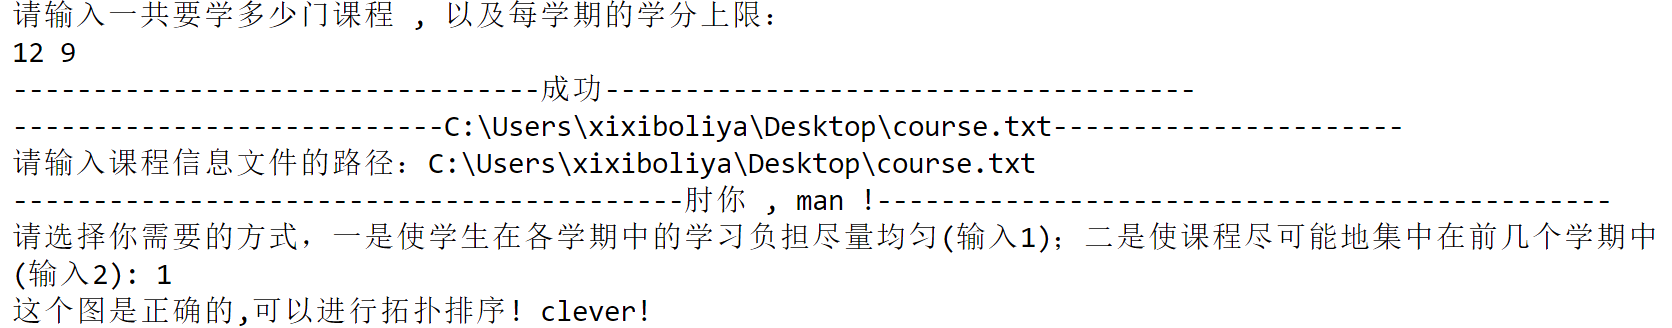
\includegraphics[width=0.8\textwidth]{6027.png}
    \caption{界面}
    \label{fig:jiemian}
\end{figure}
    \subsection{输入}
    采用记事本输入,并对输入中的注释进行了去除操作,采用fget()和 ungetc()函数读取一个字符看一看是不是‘/’或回车,是的话放回并丢弃该行。
\begin{figure}[h]
    \centering
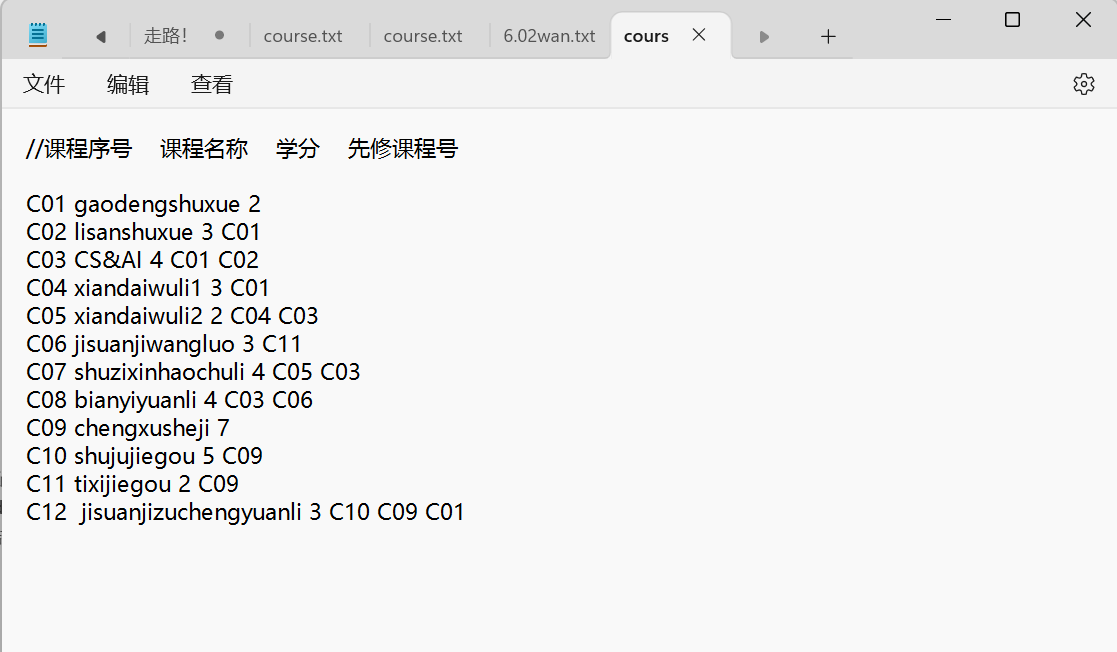
\includegraphics[width=0.9\textwidth]{6023.png}
    \caption{输入界面}
    \label{fig:enter}
\end{figure}
\vspace{0.5cm}
    \subsection{均匀排课}
    \begin{figure}[H]
    \centering
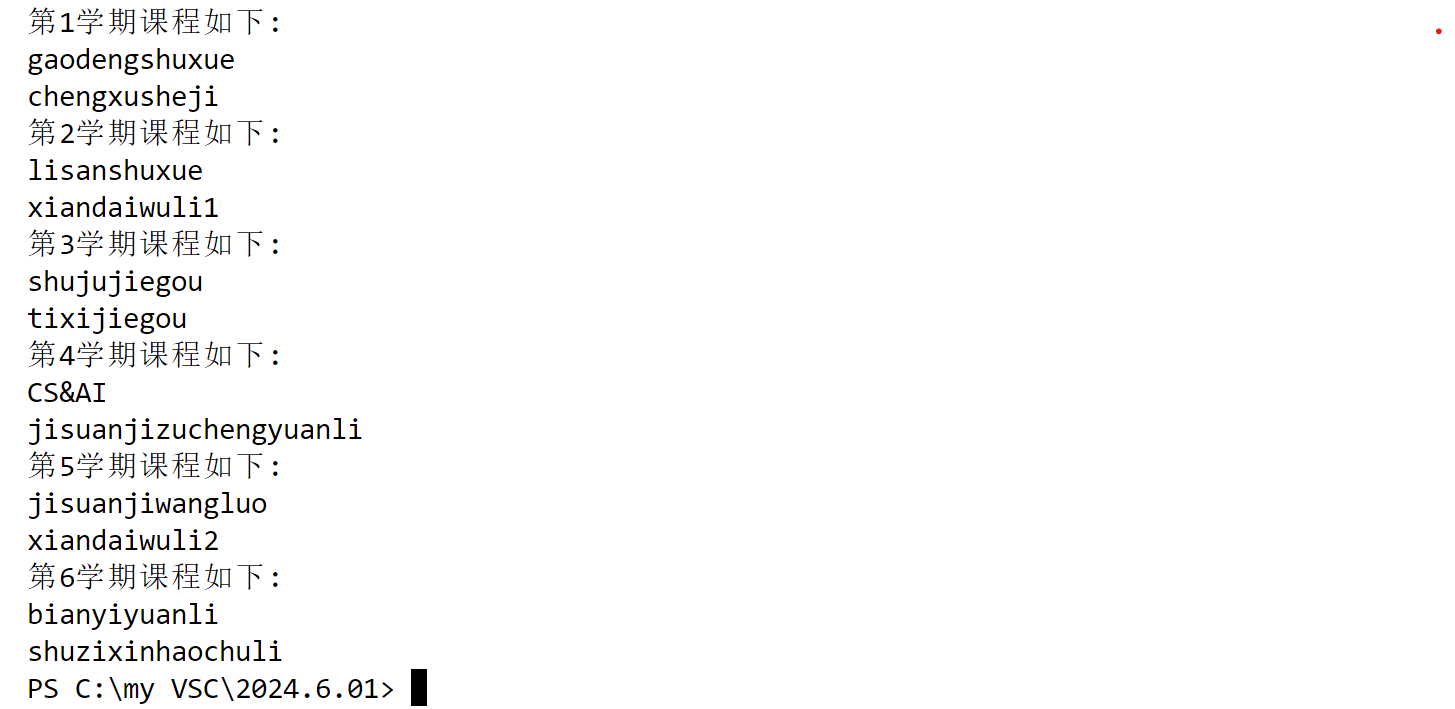
\includegraphics[width=0.8\textwidth]{6026.png}
    \caption{均匀排课}
    \label{fig:junyun}
\end{figure}
\vspace{0.5cm}
    \subsection{集中排课}
    \begin{figure}[H]
    \centering
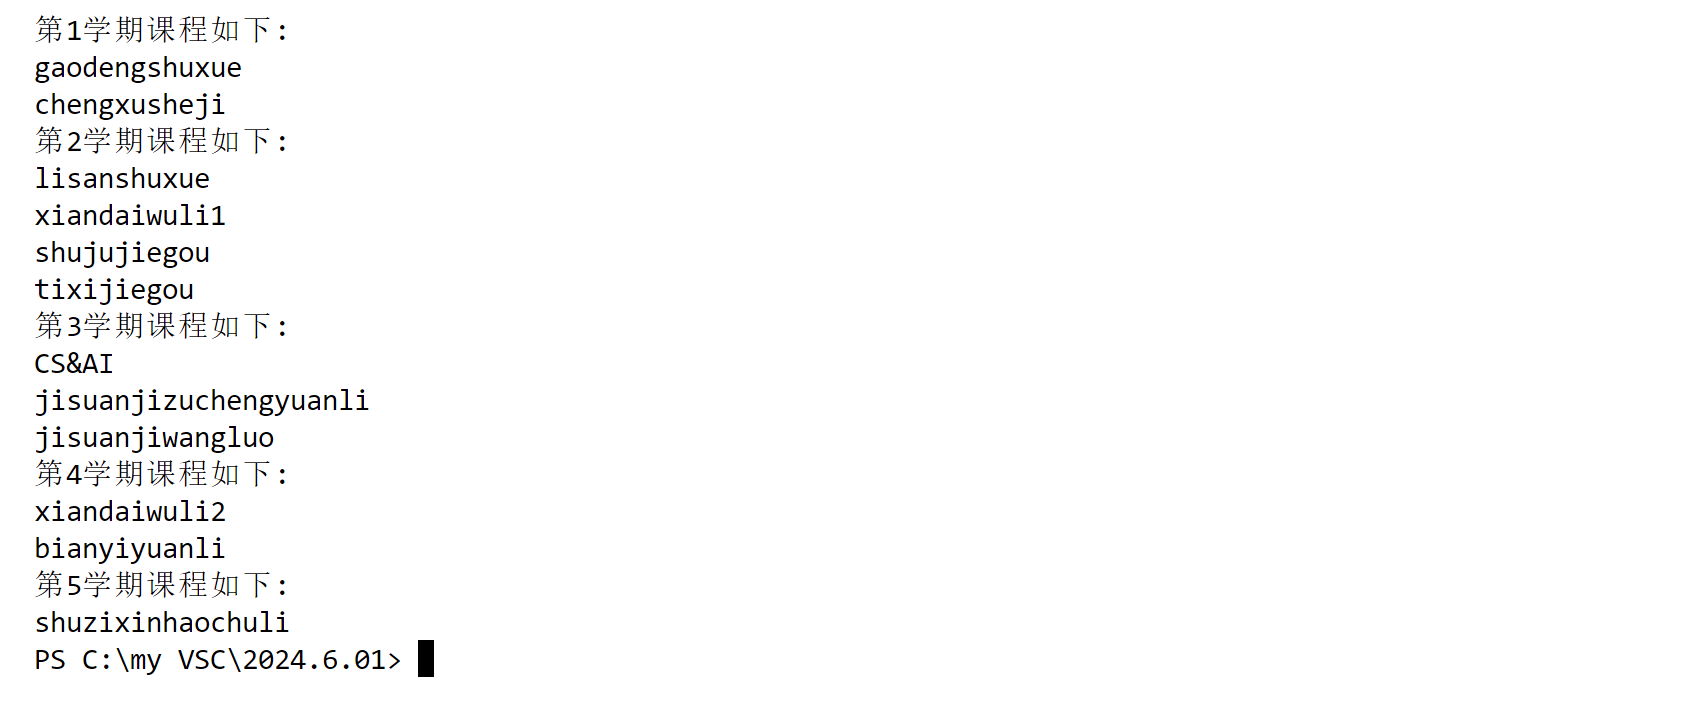
\includegraphics[width=0.8\textwidth]{6025.png}
    \caption{集中排课}
    \label{fig:enter-label}
\end{figure}
可以看到,这两种排课方式对于第六学期的安排并不相同,说明两个拓扑排序的代码都管用。
\section{实验总结}
  \subsection{收获}
  \begin{enumerate}
      \item {学会了因为多个cpp文件联合使用而修改setting.json文件的方法}
      \item {初步掌握了用\LaTeX{}写文档的方法}
      \item {对防止野指针的出现做出了顽强的挣扎}
      \item {对输入进行了创新,从记事本中读入数据并且去掉注释}
  \end{enumerate}
  \subsection{存在的问题}
    \begin{enumerate}
      \item {程序健壮性较弱,不能对不法输入进行assert警告,虽然使用了exit(1)进行一定的修补}
      \item {对相关类的规定仍然不太清楚,感觉可以将Graph类和ClassTable类分开装进两个cpp文件里}
      \item {对类内、外函数进行的区分完全根据实际需要确定,没有太多逻辑}
  \end{enumerate}

 % \pgfplotstabletypeset[ col sep=comma, string type, every head row/.style={before row=\toprule, after row=\midrule}, every last row/.style={after row=\bottomrule}, ]{filename__1.csv}
\end{document}
